\section{Grundlagen und Begriffserklärungen}

\subsection{Die Composable-Enterprise-Architektur}

\subsubsection{Begriffserklärung und Abgrenzung}
\label{sec:CEA_B}
Flexibilität, Resilienz und Agilität. Nach Ansicht von Steve Denning, Managementberater und Autor der Forbes, sind dies Eigenschaften, in welchen sich \enquote{erfolgreiche von erfolglosen Unternehmen unterscheiden} \cite{Denning.20170210}. Für Analystenhäuser wie Gartner stet dabei fest, dass es technologischer Innovation benötigt, um einhergehende Herausforderungen erfolgreich zu bewältigen und eine kontinuierliche Unternehmenstransformation voranzutreiben. Gartner empfiehlt dabei monolithische und starre Unternehmensarchitekturen, durch einen modularen Organisationsaufbau zu ersetzen. In seinen Veröffentlichungen verwendet Gartner für dieses Konzept den Begriff der \textbf{\ac{CEA}}.
\begin{center}
	\begin{figure}[H]
		\centering
		\scalebox{0.3}{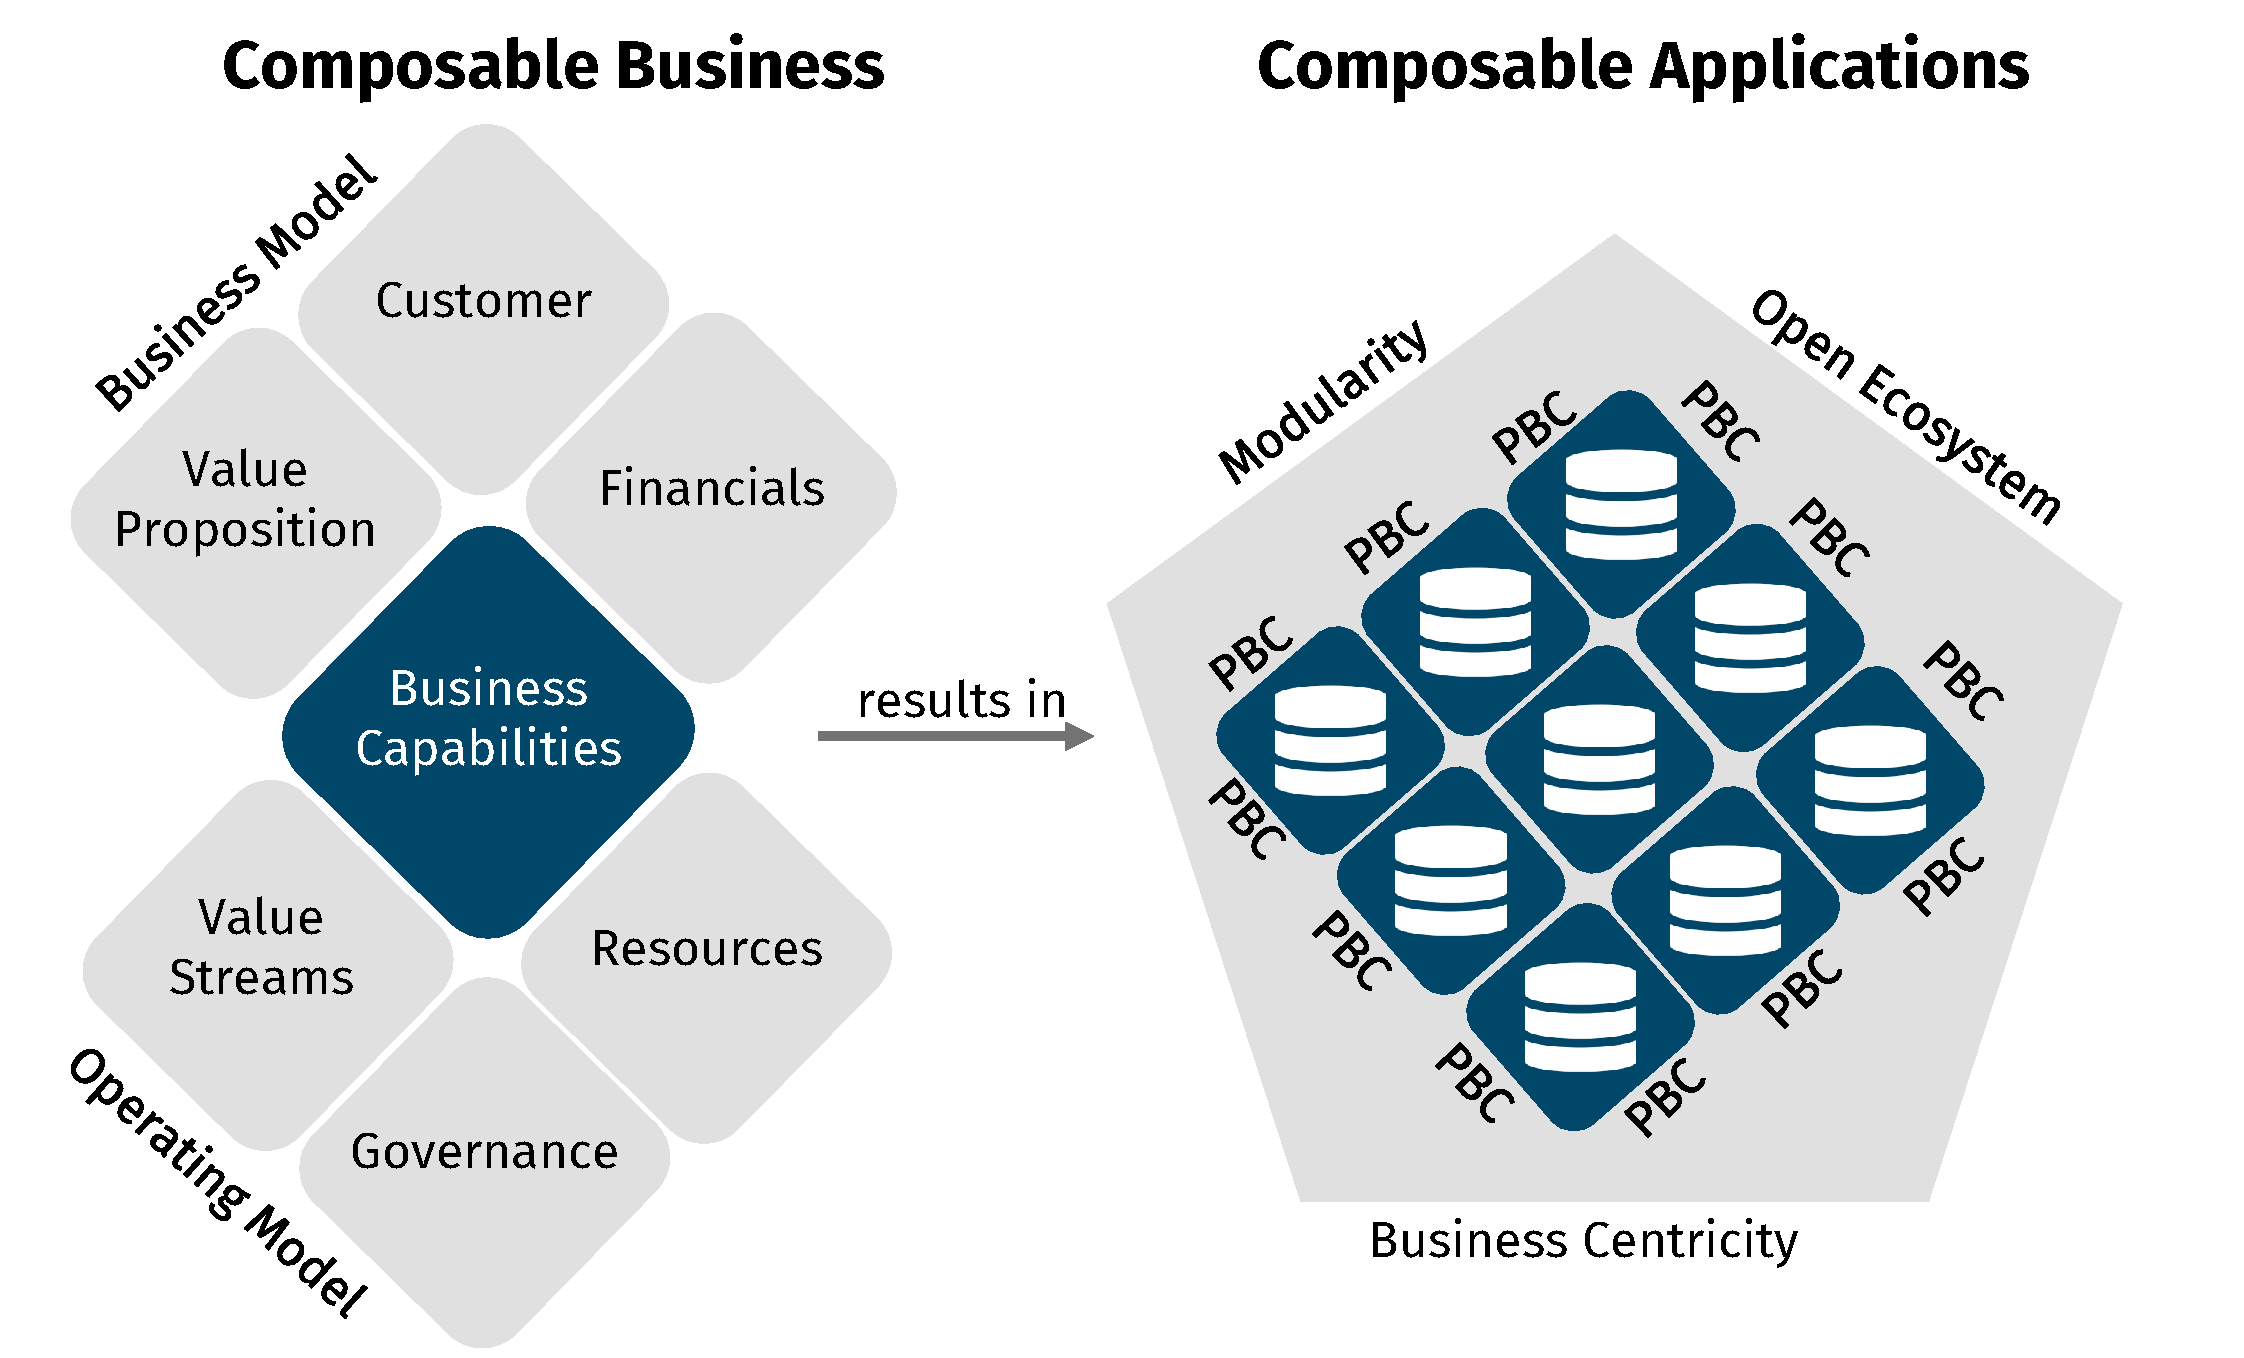
\includegraphics{CEA}}
		\caption[Entstehung einer Composable-Enterprise-Architektur]{Entstehung einer Composable-Enterprise-Architektur. In Anlehnung an Schönstein \cite{Schonenstein.20230103}.}
		\label{fig:CEA}
	\end{figure}	
\end{center}
\vspace*{-15mm}
In der Literatur wird die CEA dabei wie folgt definiert:\vspace{2mm}\\
\textit{\enquote{The Composable-Enterprise-Architecture is an architecture that delivers business outcomes and adapts to the pace of business change. It does this through the assembly and combination of packaged business capabilities \cite{.20230313}.}}\vspace{2mm}\\
Ein Composable-Enterprise ist somit ein aus mehreren Bausteinen, sog. \textit{\ac{PBC}} bestehendes Unternehmen. PBCs sind vorgefertigte Softwareelemente, welche jeweils eine bestimmte Geschäftsfunktion abdecken (s. Abb. \ref{fig:CEA}).
Damit ein Unternehmen zu einem \ac{CE} wird, muss dieses drei Grundsätze einhalten: \textit{Modulare Architektur}, \textit{Offenes Ökosystem} und \textit{Businesszentriertheit} \cite{.20230313}. Laut Gartner müssen Unternehmen nicht nur \enquote{akzeptieren, dass der disruptive Wandel zur Normalität gehört}. Vielmehr sollten diese den disruptiven Wandel als \enquote{Chance begreifen und ihn nutzen, um eine \textit{modulare Architektur} zu implementieren} \cite{.20230313}. Ergibt sich eine Änderung in den Geschäftsanforderungen, ermöglicht diese Architektur ein flexibles und isoliertes Austauschen, Verändern sowie Weiterentwickeln einzelner PBCs. Um eine auf den Geschäftszweck maßgeschneiderte IT-Lösung zu implementieren, werden diese spezialisierten Komponenten kombiniert und miteinander verknüpft \cite[315]{Chang.1019202010232020}. So kann ein Composable-E-Commerce-Enterprise Elemente, wie den Warenkorb, die Produktsuche oder die Zahlungsabwicklung in modulare Systeme auslagern. Bei Expansion in das Ausland, könnte das Unternehmen benötigte Komponente, wie z.B. PBCs zur Abwicklung von Auslandszahlungen integrieren, ohne dabei umfassende Systemänderungen durchführen zu müssen. Das Prinzip des \textit{offenen Ökosystems} ermöglicht Anwendern und Entwicklern Werkzeuge, welche zur Unterstützung der operativen Tätigkeiten benötigt werden, selbst zusammenzustellen und frei zu kombinieren. Die in dem offenen Ökosystem integrierbaren Tools werden dabei auf einem Marktplatz gebündelt und können ohne hohen Aufwand aktiviert und unmittelbar bereitgestellt werden \cite[58]{.2009}. Dazu gehören etwa Tools zur Automatisierung von Prozessen oder Kollaborationsdienste zur Unterstützung der Zusammenarbeit innerhalb von Teams. Neben diesen administrativen Werkzeugen werden auf Marktplätzen ebenfalls offene Technologiestandards, wie Datenbanken oder Sicherheitstools angeboten. Diese werden von CEs als Werkzeuge zur Unterstützung der Anwendungsentwicklung verwendet. Mit der Nutzung solcher externen Standards, Services und Tools können CEs die eigenen Fähigkeiten im Bereich der nicht-kerngeschäftlichen Kompetenzen erweitern und somit Wettbewerbsvorteile erlangen \cite[7]{Sensedia.2020}. Um eine anwenderzentrierte Gestaltung der auf dem Marktplatz angebotenen Werkzeuge zu ermöglichen, sollte der Fokus dieser Tools auf den Bedürfnissen und Erwartungen der Nutzer liegen (\textit{Businesszentriertheit}). IT-Systeme dienen dem Zweck der Unterstützung operativer Aufgaben. Entsprechen diese nicht den Anforderungen der Nutzer kann dies zu Ineffizienzen innerhalb der Arbeitsprozesse führen. Deshalb ist essenziell, dass Mitarbeiter Systeme intuitiv nutzen und ggf. weiterentwickeln und anpassen können, ohne dabei von der IT-Abteilungen abhängig zu sein \cite{.20230313}. 

\subsubsection{Technologische Konzepte des Composable-Enterprises}
Um die in Kapitel \ref{sec:CEA_B} aufgeführten betriebswirtschaftlichen Grundsätze in das eigene Unternehmen zu integrieren, benötigt es verschiedener technologischer Konzepte. Zusammenfassen lassen sich diese mit dem Akronym \textit{MACH}: \textit{\acl{MACH}}.
\begin{center}
	\begin{figure}[H]
		\centering
		\scalebox{0.4}{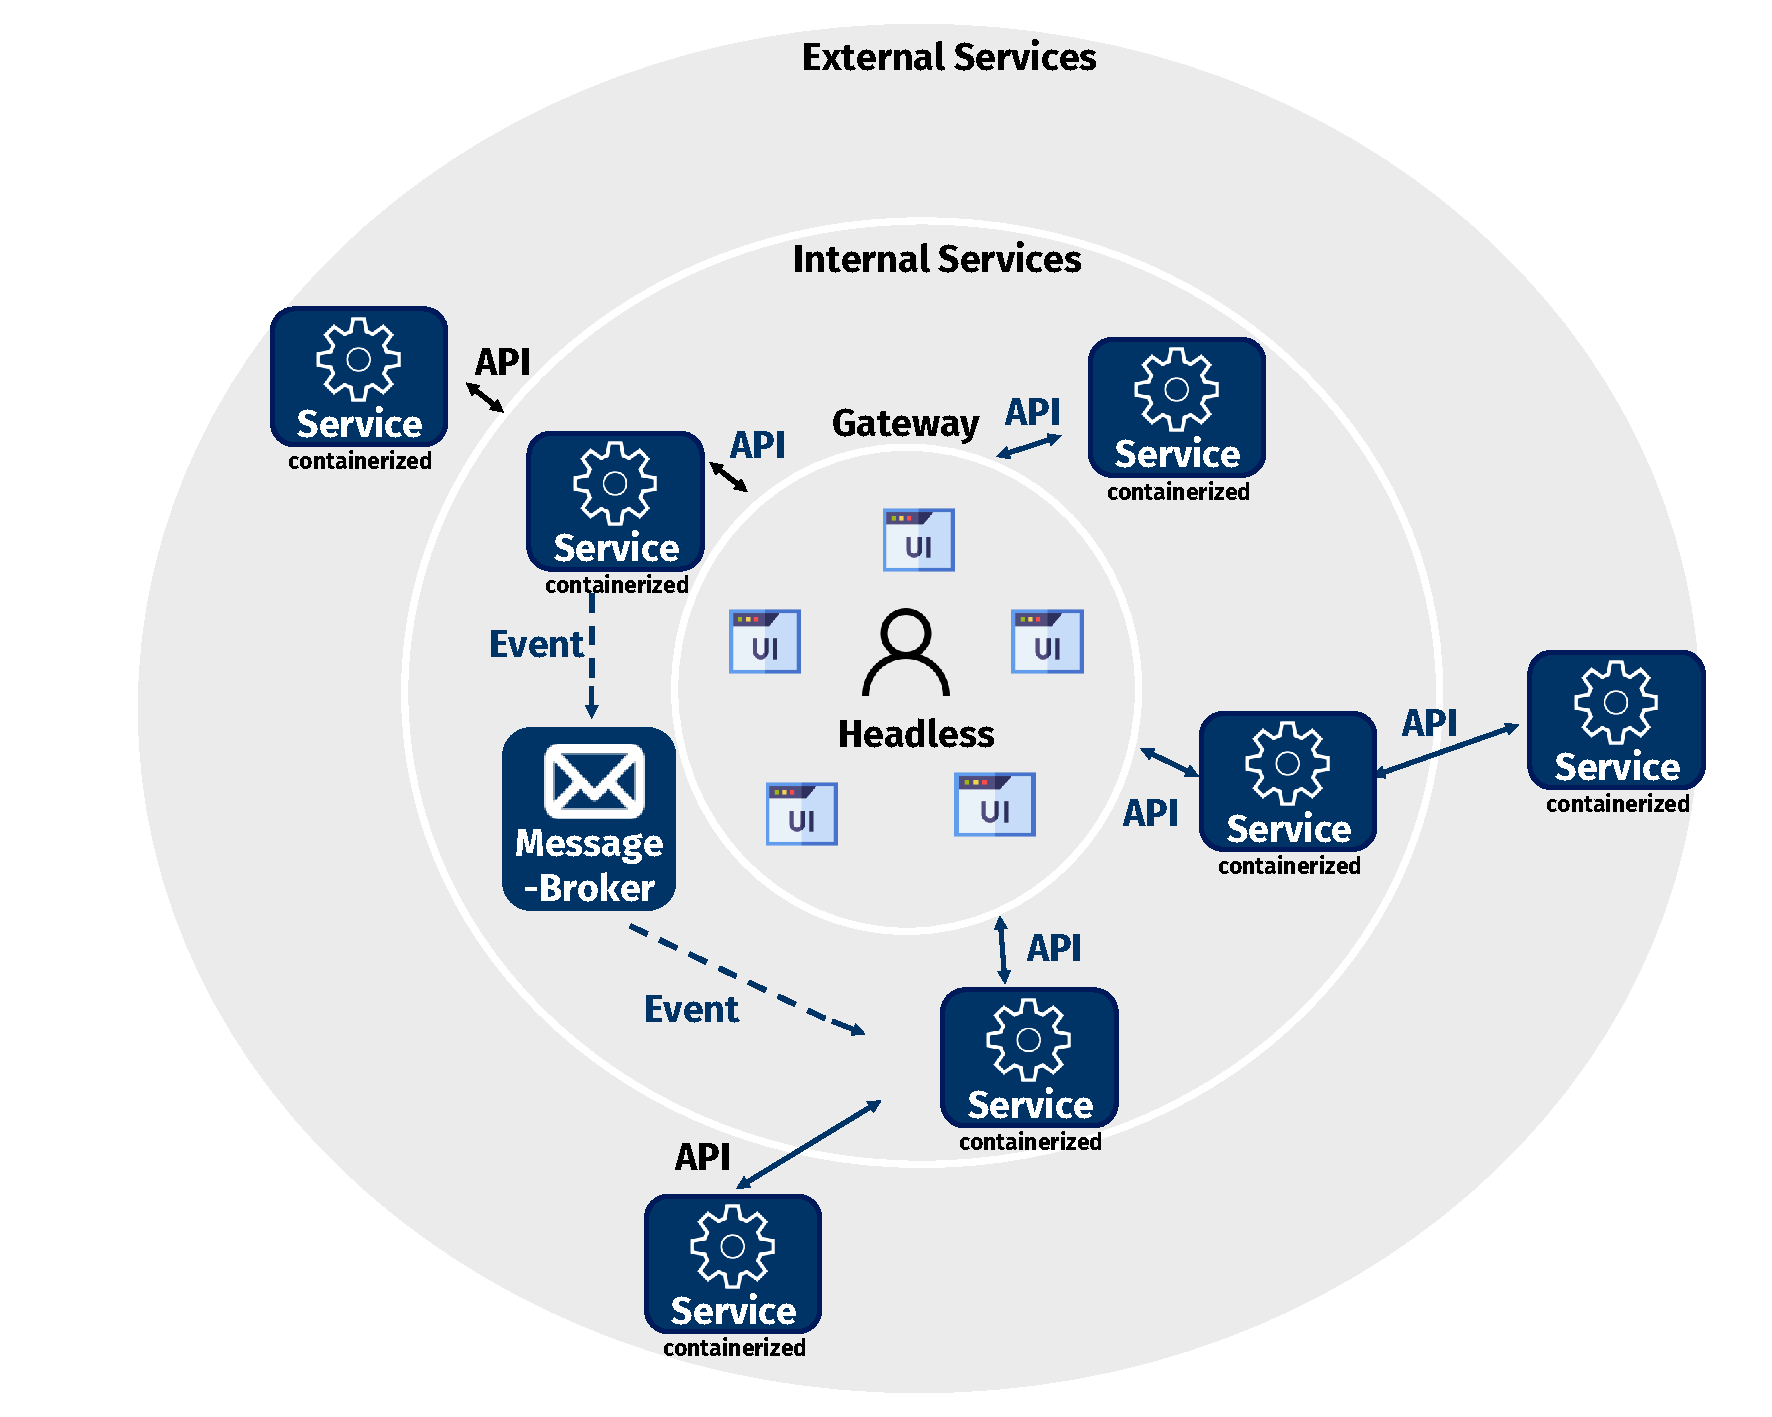
\includegraphics{CEA_K}}
		\caption[Technische Realisierung der Composable-Enterprise-Architektur]{Technische Realisierung der Composable-Enterprise-Architektur. Eigene Darstellung.}
		\label{fig:CEA_K}
	\end{figure}	
\end{center}
\vspace*{-15mm}
Der zentrale Einstiegspunkt des Nutzers (Client) in einer CE-Anwendung ist das User-Interface. Insbesondere für Content-Management-Systeme wird für Frontend-Entwicklungen das \textit{Headless-Konzept} verwendet. Dieses beschreibt, dass zwischen Front- und Backend keine feste Kopplung besteht. Vielmehr werden auf dem Backend standardisierte Daten verwaltet, welche auf verschiedenen Frontends ausgegeben werden können \cite{.20230313}. Die Applikationslogik des Backends wird dabei in kleine isolierte \textit{Microservices} gekapselt. Um Nachrichten zwischen Frontend und den Services zu übermitteln, wird i.d.R. ein Gateway zwischengeschaltet \cite[41]{.2009}. Mit diesem wird eine zentrale und standardisierte Schnittstelle bereitgestellt, welche verschiedene Authentifizierungs-, Autorisierungs- sowie Routing-Mechanismen implementiert. Die einzelnen Services werden auf losen Instanzen betrieben, welche jedoch im Zusammenspiel eine große Anwendung darstellen. Dabei ist möglich, für jeden Service eine unterschiedliche Programmiersprache sowie Datenbank zu verwenden. So können Architektur und Technologien eines Services unmittelbar an dessen betriebswirtschaftliche Anforderungen angepasst werden.
Zur Kommunikation zwischen Services werden standardisierte Schnittstellen, sog. \textit{\ac*{APIs}} verwendet. Mit APIs werden die von den Services bereitgestellten Funktionalitäten und Daten veröffentlicht \cite[15]{Biehl.2015}. Diese Schnittstellen können dabei unmittelbar von dem Frontend oder anderen Microservices konsumiert werden. Zur Implementierung von APIs werden dabei i.d.R. Protokolle wie HTTP oder OData verwendet. Ein weiteres bei CEs verwendetes Kommunikationskonzept ist die \textit{\ac{EDA}}. Während APIs auf konkrete Serviceanfrage wie z.B. HTTP-GET-Requests reagieren, bezweckt die \acs{EDA} eine asynchrone Verarbeitung von Events. Dabei werden einzelnen Services die Rollen eines \textit{Event Producers} bzw. \textit{Event Consumers} zugewiesen \cite[51]{Bruns.2010}. Der Event Producer erzeugt Nachrichten und übermittelt diese einer unabhängigen Instanz zur Verwaltung der Events (\textit{Message Broker}) \cite[61]{Bruns.2010}. Ein Event Consumer kann dabei bestimmte Themen des Message Brokers abonnieren und  gesendete Ereignisse auslesen bzw. verarbeiten \cite[54]{Bruns.2010}. Da der Message Broker eine unabhängige Vermittlungsinstanz zwischen den Services darstellt, können neue Dienste Event-Themen abonnieren und somit ohne hohen Aufwand in eine bestehende Kommunikation eingegliedert werden. Alle Komponenten der CEA werden auf einer Cloud-Plattform betrieben (\textit{cloud-native}). Cloud-Computing ist ein Dienstleistungsmodell, welches Nutzern ermöglicht Ressourcen, wie Speicher, Analyse-Tools oder Software über das Internet von einem Cloud-Anbieter zu beziehen \cite[5]{Reinheimer.2018}. Für das Cloud-Computing werden durch das \ac{NIST} verschiedene Servicemodelle definiert. Neben \textit{\ac{SaaS}} und \textit{\ac{IaaS}}, bei welchem  eine Anwendung bzw. eine gesamte Infrastruktur in der Cloud gemietet wird, gibt es ebenfalls das \textit{\ac{PaaS}} \cite{Reinheimer.2018} \cite[9]{Reinheimer.2018}. Bei diesem Computing-Modell wird eine Plattform bereitgestellt, auf welcher Kunden eigene Anwendungen entwickeln, testen und betreiben können. Ein auf dieser Service-Ebene von der SAP bereitgestelltes Produkt ist die SAP \acl{BTP} (SAP \acs{BTP}). Diese stellt eine Reihe von Diensten und Funktionen zur Verfügung, mit welchen Kunden die eigenen SAP-ERP-Systeme anpassen, integrieren und erweitern können. PaaS ermöglicht IT-Services schnell und kosteneffizient an aktuelle Markterfordernisse anzupassen. Aufgrund der nutzungsabhängigen Bepreisung von Cloud-Plattformen können Dienste ohne hohen Investitionseinsatz auf- und abgebaut werden. Da Services in Cloud-Plattformen i.d.R. auf virtuellen bzw. containerisierten Umgebungen betrieben werden, können Anwendungen schnell und effizient skaliert und somit stets die benötigte Rechenleistung bereitgestellt werden \cite[10]{Reinheimer.2018}. 

\subsection{Integration und Bereitstellung von Software}
\subsubsection{Agile und DevOps als moderne Anwendungsentwicklungskonzepte}
Das Hauptaugenmerk eines CEs besteht darin eine möglichst modulare und flexible Systemarchitektur zu schaffen. Damit soll sichergestellt werden, dass IT-Leistungen in einem sich stetig ändernden Umfeld schnell und risikoarm bereitgestellt werden. Das traditionelle Wasserfallmodell, welches eine sequenzielle Abfolge der Projektelemente \textit{Anforderung}, \textit{Design}, \textit{Implementierung}, \textit{Test} und \textit{Betrieb} vorgibt, besitzt dabei signifikante Limitationen. Die in dieser Methodik detailliert durchgeführte Vorabplanung, kann insbesondere in umfangreichen Langzeitvorhaben aufgrund unvorhersehbarer Externalitäten selten eingehalten werden. Auch die starre Abfolge der Projektphasen mindert insbesondere in fortgeschrittenen Zeitpunkten des Vorhabens den Spielraum für Anpassungsmöglichkeiten \cite[5]{Vivenzio.2013}. Dies resultiert nicht nur einem Anstieg der Kosten, sondern führt ebenfalls dazu, dass IT-Projekte länger als geplant ausfallen \cite[41]{Vieweg.2015}. Als Reaktion haben sich innerhalb der Projektmanagementlandschaft zunehmend \textbf{agile Vorgehensmodelle} etabliert.
Im Gegensatz zum Wasserfallmodell, welches eine umfassende Vorabplanung vorsieht, wird das Vorhaben in einer agilen Entwicklung in viele zyklische Einheiten, sog. \textit{Sprints}, segmentiert (s. Abb. \ref*{fig:Agile_Cycle}) \cite[87]{Goll.2015}. Alle innerhalb des Projektumfangs zu entwickelnden Funktionalitäten werden dabei in einem zentralen Artefakt (\textit{Product Backlog}) festgehalten und von dem Produktverantwortlichen (\textit{Product Owner}) priorisiert. 
\begin{center}
	\begin{figure}[H]
		\centering
		\scalebox{0.5}{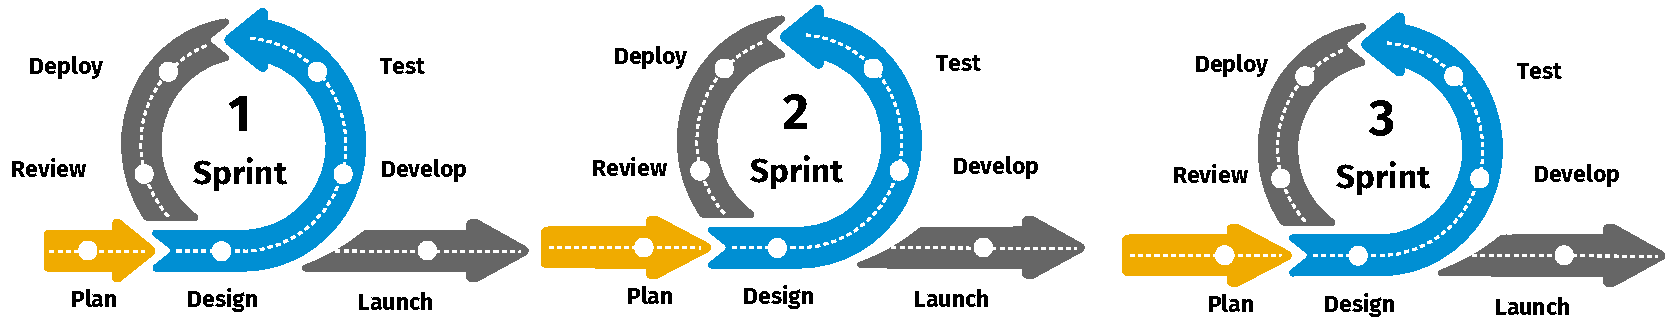
\includegraphics{Agile_Cycle}}
		\caption[Exemplarische Abfolge eines agilen Entwicklungszykluses]{Exemplarische Abfolge eines agilen Entwicklungszykluses. In Anlehnung an K\&C \cite{K&C.2021}.}
		\label{fig:Agile_Cycle}
	\end{figure}	
\end{center}
\vspace*{-15mm}
Sprints sind Durchläufe, welche i.d.R. einen Zeitraum von ein bis vier Wochen umfassen. Während dieses Abschnitts ist die Fertigstellung einer vor dem Sprint definierten Aufgabenkontingente (\textit{Sprint Backlog}) vorgesehen. Nach Abschluss eines Sprints soll dabei ein potenziell an den Kunden auslieferbares Produkt zur Verfügung gestellt werden. Dies erlaubt eine schnelle Bereitstellung funktionsfähiger Software, was neben einem beschleunigtem Kundennutzen ebenfalls in einer Optimierung der Planungsprozesse resultiert. So kann das nach Ablauf eines Sprints an die Stakeholder ausgelieferte Artefakt als Feedback-Grundlage verwendet und im unmittelbaren Folge-Sprint eingearbeitet werden \cite[39]{K&C.2021}.
Innerhalb der letzten Dekade haben sich diverse auf agilen Prinzipien basierenden Vorgehensmodelle, wie Scrum, Kanban oder \ac{XP} in der Softwareentwicklung etabliert. Obwohl einige dieser Methoden zur erfolgreichen Zusammenarbeit innerhalb der Entwicklungsteams beigetragen haben, bleibt das sog.  \textit{Problem der letzten Meile} bestehen \cite{Qentelli.20230305}. Traditionell erfolgt eine funktionale Trennung der Entwickler- und IT-Betriebler-Teams. Das Problem der letzten Meile beschreibt dabei, dass aufgrund ausbleibender Kooperation der Entwicklungs- und Betriebsteams der Programmcode nicht auf die Produktivumgebung abgestimmt ist. Erkenntnisse aus der Praxis zeigen, dass solche organisatorischen Silos häufig in einer schlechten Softwarequalität und somit in einem geminderten Ertragspotenzial bzw. in einer Erhöhung der Betriebskosten resultieren \cite[1]{Halstenberg.2020}. So geht aus der von McKinsey veröffentlichen Studie \textit{The Business Value of Design 2019} hervor, dass durchschnittlich 80 Prozent des Unternehmens-IT-Budgets zur Erhaltung des Status quo, also zum Betrieb bestehender Anwendungen verwendet wird. Stattdessen fordert das Beratungshaus eine Rationalisierung der Bereitstellung von Software, um finanzielle Mittel für wertschöpfende Investitionen zu maximieren \cite{.20230305}. Abhilfe schaffen kann das in der Literatur als \textbf{\ac{DevOps}} bekannte Aufbrechen organisatorischer Silos zwischen Entwicklung und dem IT-Betrieb \cite[1]{Halstenberg.2020}. 
Dabei stellt DevOps keine neue Erfindung dar. Stattdessen werden einzelne bereits bewährte Werkzeuge, Praktiken und Methoden, wie z.B. die agile Softwareentwicklung, zu einem umfassenden Rahmenwerk konsolidiert. DevOps zielt dabei auf eine Optimierung des gesamten Applikationslebenszykluses, von Planung bis Bereitstellung der Software, ab. Neben der Bereitstellung von IT-Services umfasst DevOps ebenfalls Aktivitäten zu IT-Sicherheit, Compliance und Risikomanagement. Prägnant zusammenfassen lässt sich das DevOps-Konzept durch das Akronym CAMS: \textit{Culture (Kultur)}, \textit{Automation (Automatisierung)}, \textit{Measurement (Messung)} und \textit{Sharing (Teilen)} \cite[5]{Halstenberg.2020}. Dabei gilt \textit{Kultur} als das wohl wesentlichste DevOps-Erfolgselement. Diese bezweckt eine Kollaborationsmentalität, welche sich über alle Ebenen eines Unternehmens erstreckt. Operative Entscheidungen sollen dabei auf die Fachebenen herunter delegiert werden, welche aufgrund ihrer spezifischen Expertise am geeignetsten sind, Dispositionen zu verabschieden \cite[5]{Halstenberg.2020}. Eine \textit{Automatisierung} der Softwarebereitstellungsprozesse ermöglicht, sich wiederholende manuelle Arbeit zu eliminieren. Dies kann ebenfalls zur Rationalisierung und damit zur Senkung der IT-Betriebskosten beitragen. Der dabei erzielte Einfluss wird anhand verschiedener DevOps-Kennzahlen bemessen (\textit{Messung}). Neben der Systemverfügbarkeit und der Instandsetzungszeit sind für Softwareentwicklungsunternehmen insbesondere \textit{Time-to-Market} sowie \textit{Time-to-Value} signifikante Metriken \cite[7]{Halstenberg.2020}. 
\begin{center}
	\begin{figure}[H]
		\centering
		\scalebox{0.34}{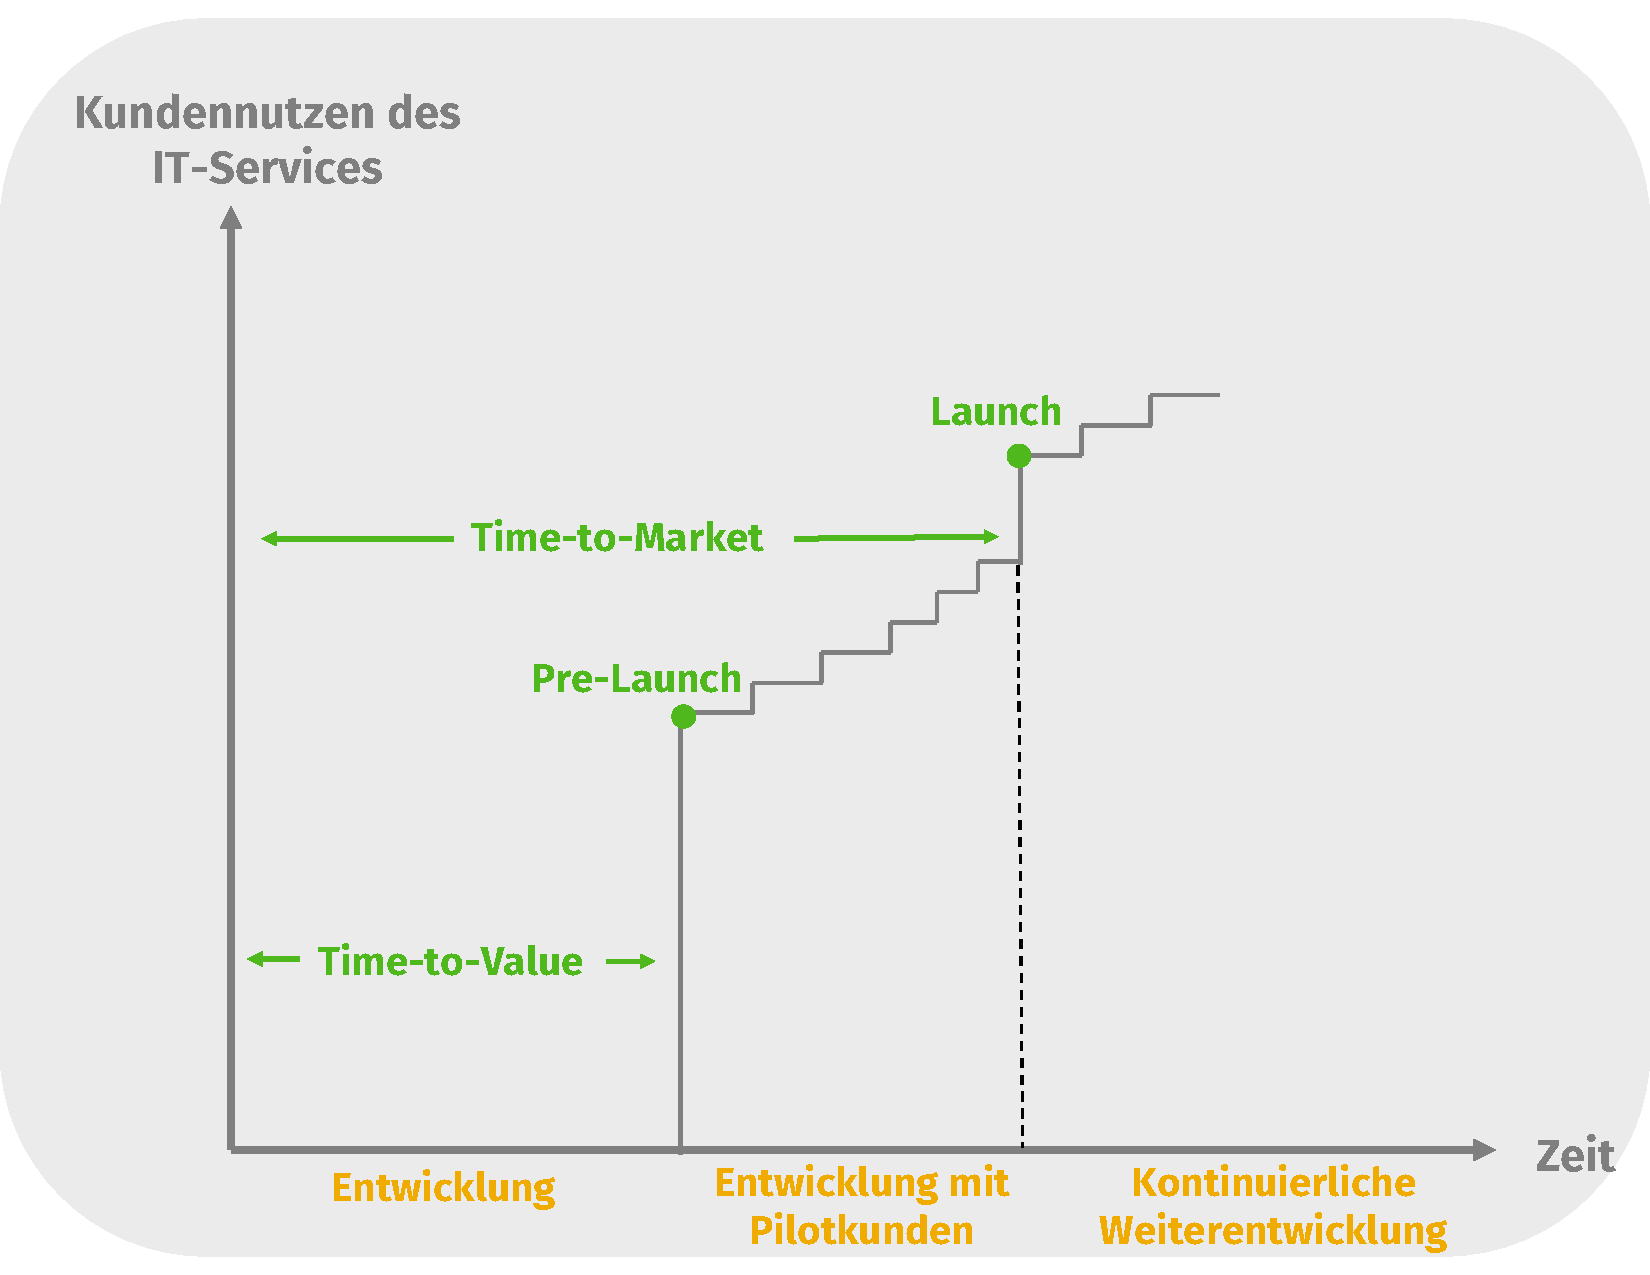
\includegraphics{TTM}}
		\caption[Zeitliche Darstellung der Herbeiführung von Kundennutzen bei der Entwicklung von IT-Services]{Zeitliche Darstellung der Herbeiführung von Kundennutzen bei der Entwicklung von IT-Services \cite[9]{Halstenberg.2020}.}
		\label{fig:TTM}
	\end{figure}
\end{center}
\vspace*{-15mm}
Der Time-to-Market beschreibt die Zeitspanne zwischen Entwicklungsentstehungsprozess und der Markteinführung von IT-Services \cite[141]{Vesey.1992}. Auch der \textit{Time-to-Value} erhält zunehmend Bedeutung in der Softwareentwicklung. Im Gegensatz zum Time-to-Market wird hier nicht die Zeit bis zur Komplett-Einführung, sondern das Intervall bis die von dem Softwareunternehmen entwickelte Lösung ersten Kundennutzen herbeiführt, bemessen. Obwohl der im Time-to-Value bereitgestellte IT-Service möglicherweise Verbesserungspotenzial besitzt, überwiegt für Kunden des Unternehmens der mit der initialen Auslieferung herbeigeführte Mehrwert. Eine solche Früheinführung ermöglicht dem Softwareunternehmen ebenfalls einen Vorsprung gegenüber Konkurrenten. So ist diesem bereits gelungen, erste Kunden zu akquirieren, deren Input und Feedback möglichst rasch erfasst und verarbeitet werden kann \cite[9]{Halstenberg.2020}. Softwareunternehmen können IT-Services ab dem Pre-Launch somit sukzessive und ressourcenoptimiert unter Zusammenarbeit mit den Pilotkunden erweitern. Auch Adam Caplan, leitender Strategieberater bei Salesforce, empfiehlt angesichts der bei Softwareintegration entstehenden Komplexität, Anwendungen schnellst möglichst in produktionsähnlichen Umgebungen zu testen \cite{Vesey.1992}. Aus diesen Erfahrungen sollen Best-Practises entwickelt werden, welche innerhalb von Teams und organisationsübergreifend weitergegeben werden (\textit{Teilen}) \cite[7]{Halstenberg.2020}. 

\subsubsection{Pipelines zur Integrations- und Bereitstellungsautomatisierung}
\label{sec:CICD}
DevOps beschreibt eine Philosophie zur Förderung der Zusammenarbeit zwischen Entwicklungs- und Betriebsteams. Ein integraler Bestandteil des DevOps-Rahmen\-werks ist \textit{\ac{CI/CD}}. CI/CD ist ein Verfahren, welches zur Verbesserung der Qualität bzw. zur Senkung der Entwicklungszeit von IT-Services beiträgt. Abhilfe schaffen soll dabei eine Pipeline, welche alle Schritte von Code-Integration bis Bereitstellung der Software automatisiert. Hauptaugenmerk liegt dabei auf einer zuverlässigen und kontinuierlichen Bereitstellung von Software \cite[471]{Zampetti.92720211012021}.
\begin{center}
	\begin{figure}[H]
		\centering
		\scalebox{0.4}{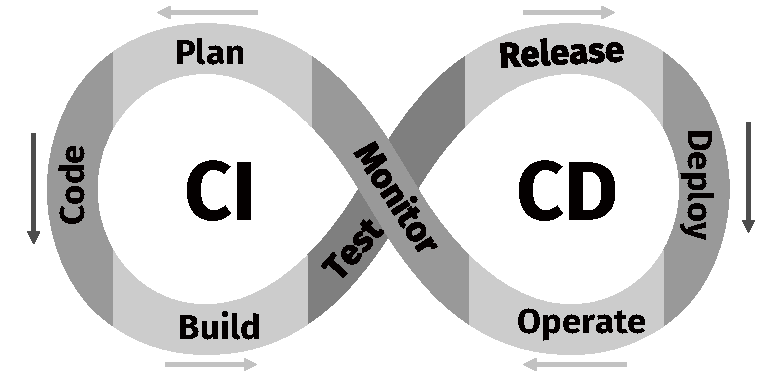
\includegraphics{CICD_Cycle}}
		\captionsetup{format=myformat}
		\caption[Aktivitäten im CI/CD-Prozess]{Aktivitäten im CI/CD-Prozess. In Anlehnung an Synopsys \cite{.20230201}.}
		\label{fig:CICD_Cycle}
	\end{figure}
\end{center}
\vspace*{-15mm}
Alle in diesem Prozess anfallenden Aktivitäten werden dabei im CI/CD-Zyklus der Abb. \ref*{fig:CICD_Cycle} dargestellt. Der \acs{CI}-Prozess (Continuous-Integration-Prozess) bezweckt, dass lokale Quellcode\-änderungen in kurzen Intervallen und so schnell wie möglich in eine zentrale Codebasis geladen werden. Das frühzeitige Integrieren von Code soll dabei zu einer unmittelbaren und zuverlässigen Fehlererkennung innerhalb des Entwicklungsvorhabens beitragen \cite[471]{Zampetti.92720211012021}. 
Der erste Schritt des CI-Prozesses umfasst die Planung zu entwickelnder Services (\textit{Plan}: s. Abb. \ref*{fig:CICD_Cycle}). Dabei soll festgestellt werden, welche Anforderungen eine Lösung besitzt bzw. welche Softwarearchitekturen sowie Sicherheitsmaßnahmen implementiert werden sollten. Um sicherzustellen, dass die in der Planung entworfene Anwendungsarchitektur auf das Design des Produktivsystems abgestimmt ist, sollte zu jedem Zeitpunkt das Know-how der Betriebsteams einbezogen werden \cite[16]{Halstenberg.2020}. Nach erfolgreichem Entwurf zu implementierender Anwendungsfeatures beginnt die Entwicklung der IT-Services (\textit{Code}: s. Abb. \ref*{fig:CICD_Cycle}). Arbeiten hierbei mehrere Entwickler parallel an demselben IT-Service, wird der entsprechende Quellcode in Versionsverwaltungssysteme (\textit{Repositorys}) wie Github oder Bitbucket ausgelagert. Ein Repository stellt dabei einen zentralen Speicherort dar, welcher das Verfolgen sowie Überprüfen von Änderungen und ein paralleles bzw. konkurrierendes Arbeiten an einer gemeinsamen Codebasis ermöglicht \cite[31]{Loeliger.2012}. Der in dem Repository archivierte Hauptzweig (\textit{Master-Branch}) stellt dabei eine aktuelle und funktionsfähige Version des Codes dar. Dieser mit verschiedenen Validierungsprozessen überprüfte Code, stellt dabei die aktuelle in dem Produktionssystem laufende Anwendungsversion dar (s. Abb. \ref*{fig:VCS}). Im Sinne der agilen Entwicklung werden dabei große Softwareanforderungen (\textit{Epics}), in kleine Funktionalitäten (\textit{User Storys}) segmentiert, welche in separate Feature-Branches ausgelagert werden. Diese sind unabhängige Kopien des Hauptzweiges, in welcher ein Entwickler Änderungen vornehmen kann, ohne Konflikte in der gemeinsamen Codebasis zu verursachen. Nach Fertigstellung der Funktionalitäten sollte der um die Features erweiterte Quellcode so schnell wie möglich in den Hauptzweig integriert werden. Da mit dieser Zusammenführungen automatische Validierungsprozesse ausgelöst werden, kann mit erfolgreicher Absolvierung der Tests sichergestellt, dass der Code stets stabil, also funktionsfähig ist und keine Konflikte mit dem aktuellen Code des Hauptzweiges aufweist \cite[169]{Loeliger.2012}. Die in diesem Schritt abgewickelten Tests leiten sich dabei aus der \textit{\ac{DoD}} ab. Die DoD ist eine in der Planungsphase festgelegte Anforderungsspezifikation, deren Erfüllung als notwendige Voraussetzung für den Abschluss eines Features gilt. Somit sind Entwickler dazu angehalten, für jedes implementierte Feature einen der DoD entsprechenden Test zu entwerfen.
\begin{center}
	\begin{figure}[H]
		\centering
		\scalebox{0.8}{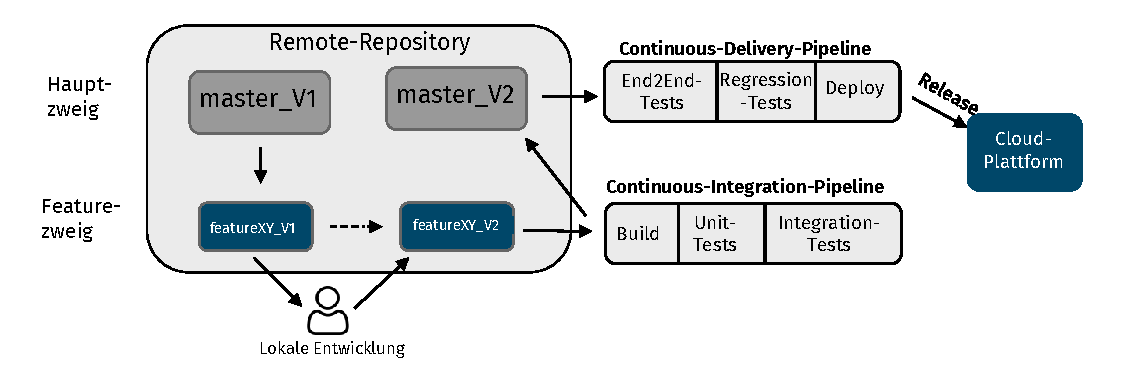
\includegraphics{VCS}}
		\caption[Versionskontrollsysteme zur Verwaltung von Quellcode]{Versionskontrollsysteme zur Verwaltung von Quellcode.\\ Eigene Darstellung.}
		\label{fig:VCS}
	\end{figure}
\end{center}
\vspace*{-10mm}
Die Einbindung des Feature-Branches in den Hauptzweig resultiert i.d.R. in einem unmittelbaren Start des \textit{CI/CD-Pipeline-Prozesses}. Bei der CI/CD-Pipeline handelt es sich dabei um eine vom Repository unabhängige Recheninstanz, welche auf einer virtuellen Maschine oder in einer containerisierten Computing-Umgebung betrieben wird \cite[Kap. 1.2]{Labouardy.2021}. Im ersten Schritt des Pipeline-Prozesses wird die Applikationen zu einem ausführbaren Programm kompiliert (\textit{Artefakt}) (\textit{Build}: s. Abb. \ref*{fig:CICD_Cycle}). Dafür können je nach Programmiersprache verschiedene Build-Tools, wie Maven für Java oder NPM für Javascript verwendet werden \cite[Kap. 7.1]{Labouardy.2021}. Nach Ablauf der Build-Workflows erfolgt eine automatische Abwicklung des Validierungsprozesses (\textit{Smoke-Tests}). Damit soll sichergestellt werden, dass zu jeder Zeit ein rudimentär getesteter Code bereitsteht und grundlegende Funktionalitäten sowie Schnittstellen erwartungsgemäß ausgeführt werden \cite[19]{Halstenberg.2020}. Der in dem Entwicklungszweig bereitgestellte Code wird dabei überwiegend anhand schnell durchführbarer Tests überprüft. Der Zweck dieser zügigen Validierungen liegt dabei insbesondere darin, dass Entwickler zeitnahes Feedback auf die Erweiterungen erhalten. So können Fehler und Konflikte so schnell wie möglich entdeckt und behoben werden, was die Entwicklung bei einer reibungslosen Auslieferung der IT-Services unterstützt. Die in der CI-Pipeline abgewickelten Validierungen umfassen i.d.R. \textit{Unit-} sowie \textit{Integration-Tests} \cite[Kap. 1.2]{Labouardy.2021}.
\begin{center}
	\begin{figure}[H]
		\centering
		\scalebox{0.3}{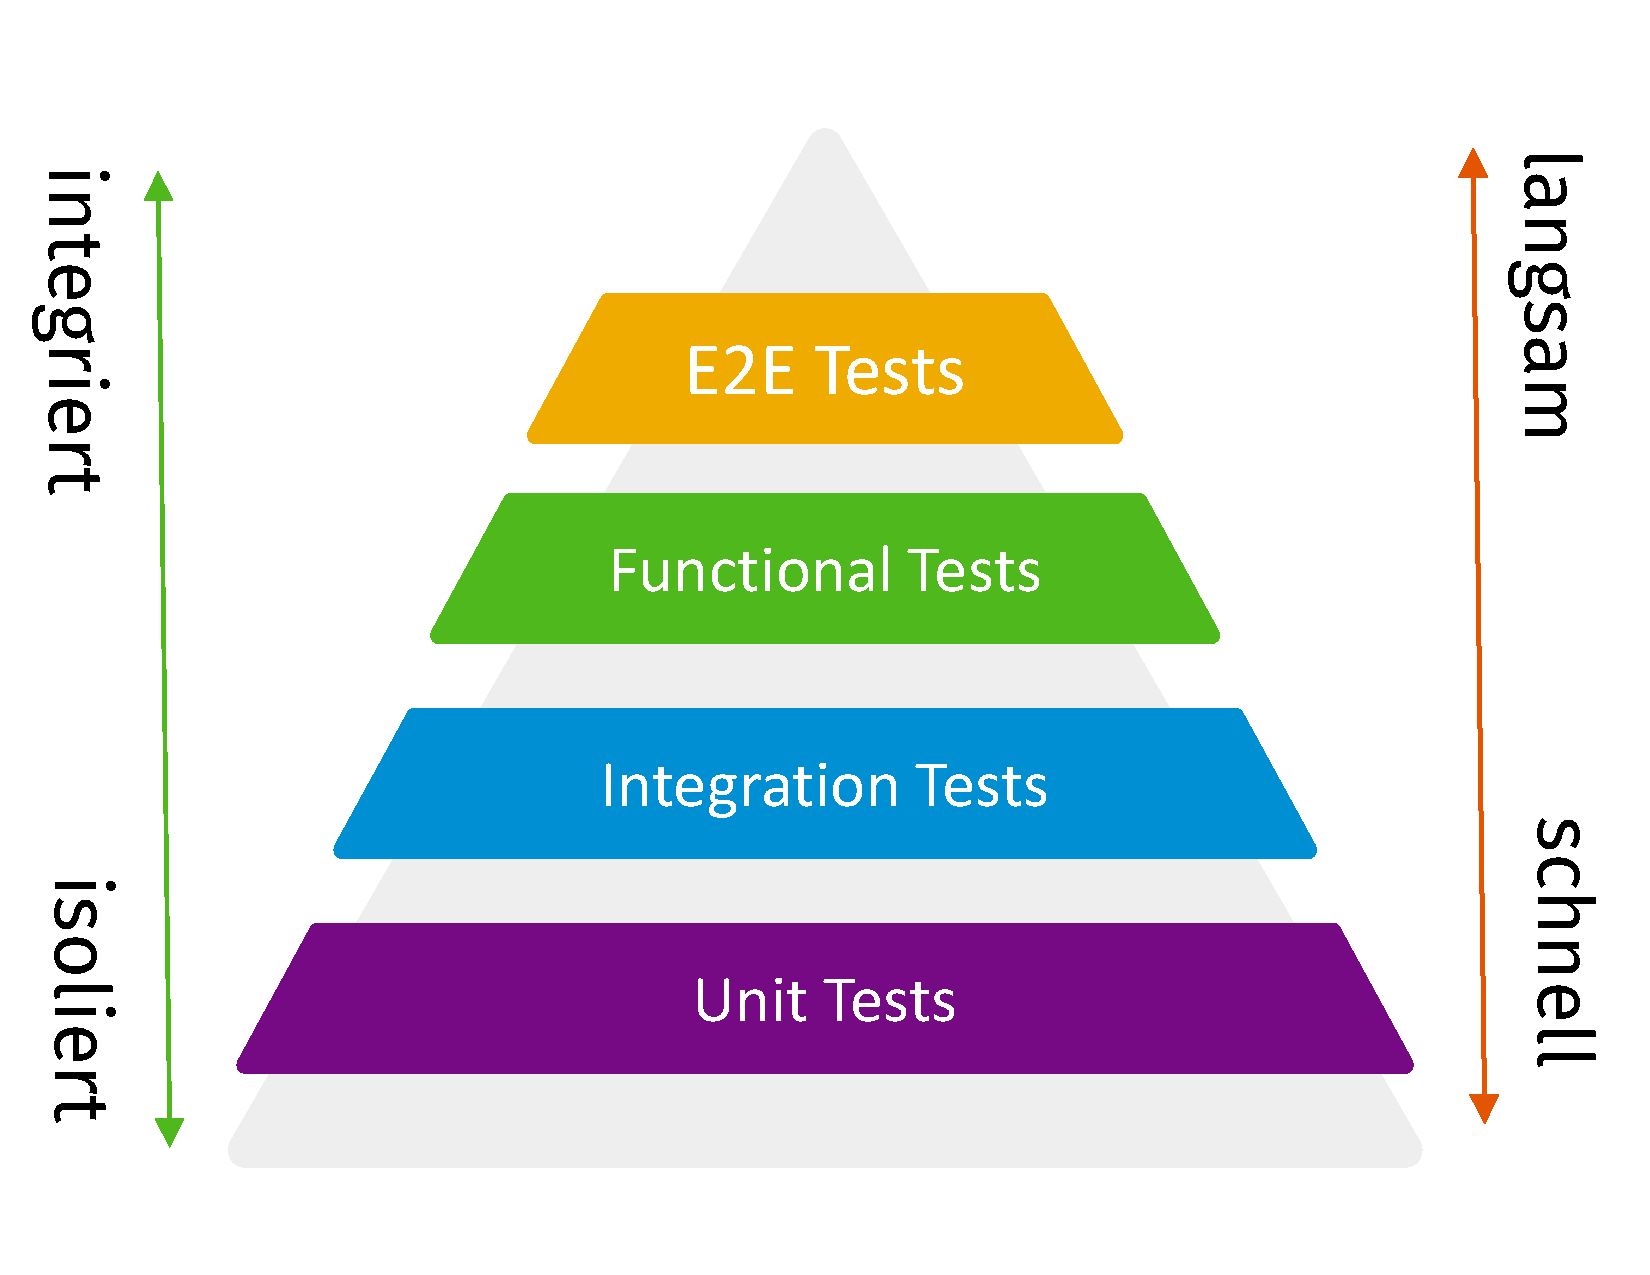
\includegraphics{Tests}}
		\caption[Hierarschische Darstellung von Softwaretests]{Hierarschische Darstellung von Softwaretests.\\ \hspace{0.5cm}In Anlehnung an Paspelava \cite{Exposit.2021}.}
		\label{fig:Tests}
	\end{figure}
\end{center}
\vspace*{-10mm}
Unit-Tests befinden sich dabei auf unterster Hierarchieebene der Test-Pyramide (s. Abb. \ref*{fig:Tests}). Somit besitzen diese eine kurze Ausführungsdauer, werden jedoch ausschließlich in einer isolierten Testumgebung abgewickelt. Mit Unit-Tests wird die funktionale Korrektheit kleinster Einheiten, wie z.B. Methoden einer Klasse, über\-prüft. Der Zweck der Unit-Tests besteht dabei in einer von externen Einflüssen und Daten unabhängigen Überprüfung der einzelnen Komponenten \cite[Kap. 2]{Hambling.2015}. Um bei der Bereitstellung neuer Funktionalitäten ebenfalls das Zusammenspiel verschiedener Komponenten zu überprüfen, werden \textit{Integration-Tests} durchgeführt. Bei diesen Tests können Aspekte, wie der Austausch eines Nachrichtenmodells zweier Web-Services oder das Response-Objekt einer Datenbankabfrage untersucht werden \cite[Kap. 2]{Hambling.2015}. Nachdem einzelne Funktionalitäten entwickelt und alle Tests erfolgreich absolviert wurden, werden die validierten Än\-derungen im Hauptzweig zusammengeführt. Mit diesem Prozessschritt beginnt der \textit{Continuous-Delivery-Workflow (\acs{CD}-Workflow)}.  Während CI den Prozess der kontinuierlichen Integration des Quellcodes in das zentrale Repository verwaltet, steuert der CD-Workflow die Automatisierung der Anwendungsbereitstellung. Applikationen sollen somit ohne große Verzögerungen in die Produktivumgebung und somit zum Kunden ausgeliefert werden. Im Sinne des DevOps-Rahmenwerkes wird der CD-Prozess automatisch und unmittelbar nach Ablauf aller CI-Aktivitäten angestoßen. In der Praxis wird hierbei jedoch häufig ein manueller Schritt zwischengeschalten \cite[20]{Halstenberg.2020}. Damit soll sichergestellt werden, dass das Ausrollen der Anwendung erst nach Überprüfung und Genehmigung der Product Owner beginnt. Im ersten Schritt des CD-Prozesses wird das in die Produktivumgebung bereitzustellende Artefakt über die Deployment-Pipeline in eine \textit{Staging-Area} geladen. Bei der Staging-Area handelt es sich dabei um ein System, welches zwischen Entwicklungs- und Produktivumgebung liegt. Die Staging-System-Konfigurationen werden dabei so angelegt, dass diese der Produktionsumgebung möglichst ähnlich sind \cite[Kap. 1.3]{Labouardy.2021}. Neben den Datenbanken werden hierbei ebenfalls Serverkonfigurationen, wie Firewall- oder Netzwerkeinstellungen von dem Produktivsystem übernommen. Somit soll sichergestellt werden, dass eine neue Anwendungsversion unter produktions-ähnlichen Bedingungen getestet wird. Analog zum CI-Prozess werden innerhalb des CD-Workflows ebenfalls Unit- und Integration-Tests abgewickelt. Diese sind i.d.R. deutlich rechenintensiver und besitzen längere Ausführungszeiten. Somit werden im CD-Prozess essenzielle, jedoch während des Entwicklungsworkflows zu aufwendige Validierungen durchgeführt \cite[20]{Halstenberg.2020}. In der Staging Area werden unterdessen auch in der Test-Pyramide (s. Abb. \ref*{fig:Tests}) höher positionierte, also rechenintensivere Tests ausgeführt \cite[Kap. 2]{Hambling.2015}. Dazu gehören \textit{Functional-Tests}. Mit diesen werden die in der Planungsphase festgelegten Anforderungen bzw. Funktionen der Anwendung überprüft. So kann z.B. evaluiert werden, ob bei Eingabe einer Benutzer-Passwort-Kennung ein korrekter Autorisierungstoken übergeben wurde. Genau wie bei Integration-Tests wird während Functional-Tests das Zusammenspiel verschiedener Komponenten überprüft. Bei Integration-Tests wird dabei jedoch lediglich die generelle Durchführbarkeit einer Kommunikation verschiedener Komponenten auf Quellcode bzw. Datenbankebene überprüft. Mit Functional-Tests wird darüber hinaus die nach Übermittlung und Prozessierung der verschiedenen Komponenten generierte Ausgabe auf Ebene des Gesamtsystems validiert. Ebenfalls während des CD-Prozesses ausgeführte Validierungen sind \textit{\ac{E2E-Tests}}. Mit diesen soll sichergestellt werden, dass die Anforderungen aller Stakeholder erfüllt werden. Hierbei wird ein vollständiges Anwenderszenario von Anfang bis Ende getestet. Dieses kann im Kontext eines E-Commerce-Webshops etwa das Anmelden mit Benutzername, das Suchen eines Produktes und das Abschließen einer Bestellung umfassen \cite{Bose.20230220}. Nachdem alle Unit-, Integration-, sowie Functional-Tests erfolgreich absolviert wurden, werden i.d.R. verschiedene Codeanalysen angestoßen. Hierbei werden Metriken, wie die prozentuale Testabdeckung oder Schwachstellen verwendeter Code-Patterns überprüft. Nach Durchführung der Codeanalysen wird das überprüfte Artefakt auf die Cloud-Plattform geladen (\textit{Deploy}: s. Abb. \ref*{fig:CICD_Cycle}). Je nach Bereitstellungsstrategie (s. \ref*{sec:Bereitstellungs_Strategien}), wird die Anwendung dann unmittelbar oder erst nach weiteren Überprüfungen für den Kunden zugänglich gemacht. Der letzte Schritt des CD-Workflows umfasst die Laufzeitüberwachung der inbetriebgenommenen Anwendung (\textit{Monitoring}: s. Abb. \ref*{fig:CICD_Cycle}). So soll eine ordnungsgemäße Ausführung der Anwendung in der Produktionsumgebung sichergestellt werden. Wichtige Überwachungselemente sind dabei \textit{Infrastruktur-}, \textit{Plattform-} sowie \textit{Anwendungs-Monitoring}. Beim Infrastruktur-Monitoring werden Metriken wie CPU-, Speicher- und Netzwerklast der Server bzw. Datenbanken untersucht. Das Plattform-Monitoring setzt dabei eine Ebene höher an und validiert, dass die Plattform, auf welcher die Anwendungen ausgeführt werden, stabil und funktionsfähig ist. Dabei werden Infrastrukturkomponenten, wie Datenbanken, virtuelle Netze bzw. Middlewares analysiert. Das Anwendungs-Monitoring umfasst die Überwachung der Funktionalitäten und der Applikation selbst. Hierbei werden Informationen wie Anfragen pro Sekunden, die Anzahl der Benutzer oder die in Log-Dateien gesammelten Fehlercodes analysiert \cite[21]{Halstenberg.2020}.\\ 
Zur Automatisierung der CI/CD-Prozesse werden bei der SAP i.d.R. drei verschiedene Pipeline-Tools verwendet. Eine unmittelbare von der SAP bereitgestellte Lösung ist das \textit{\ac{SAP CI/CD}}. Das SAP CI/CD ist eine auf der SAP BTP betriebene SaaS-Lösung, mit welcher vordefinierte Pipeline-Templates konfiguriert und ausgeführt werden können. Dieses Tool ist insbesondere mit SAP-Standardtechnologien, wie den Programmierframeworks SAP UI5 (Frontend) und SAP CAP Node (Backend) sowie der Laufzeitumgebung Cloud-Foundry kompatibel. Eine weitere bei der SAP verwendete CI/CD-Alternative ist das Open-Source-Tool \textit{Jenkins}. Im Gegensatz zum templatebasierten SAP CI/CD, muss der Bereitstellungsworkflow bei Jenkins mit der Programmiersprache Groover implementiert werden. Weiterhin wird Jenkins nicht unmittelbar auf der SAP BTP betrieben, sondern muss auf einem eigenen Server (On-Premise) oder von einem externen Cloud-Anbieter verwaltet werden. Um die Bereitstellung von SAP-spezifischen Technologien zu optimieren, wurde von der SAP die Programmbibliothek \textit{Project Piper} entworfen. Diese Bibliothek umfasst hoch konfigurierbare Implementationsschritte, Szenarien und Dienstprogramme welche für das Ausrollen von SAP-Anwendungssoftware essenziell sind.
Ein externes ebenfalls innerhalb der SAP verwendetes CI/CD-Werkzeug ist \textit{Azure Pipelines}. Azure Pipelines ist ein von Microsoft entwickeltes Tools, welches umfassende Integrationsmöglichkeiten zu anderen Microsoft-Diensten wie die Azure-Cloud-Platform oder Microsoft Visual Studio Code bietet. Zur Implementierung des CI/CD-Workflows SAP-spezifischer Technologien wird für Azure Pipelines ebenfalls die Programmbibliothek Project-Piper verwendet.
\subsubsection{Strategien zur Bereitstellung von Neuentwicklungen}
\label{sec:Bereitstellungs_Strategien}
Nachdem das Artefakt auf einer virtuellen Maschine bzw. containerisierten Cloud-Instanz installiert und gestartet wurde, erfolgt die Inbetriebnahme der neuen Anwendungsversion je nach Bereitstellungsstrategie unmittelbar oder erst nach weiteren Validierung. Anhand der Bereitstellungsstrategie wird festgelegt, mit welcher Methode und zu welchem Zeitpunkt Nutzeranfragen von der aktuellen auf die neue Anwendungsinstanz umgeleitet werden.
\begin{center}
	\begin{figure}[H]
		\centering
		\scalebox{0.4}{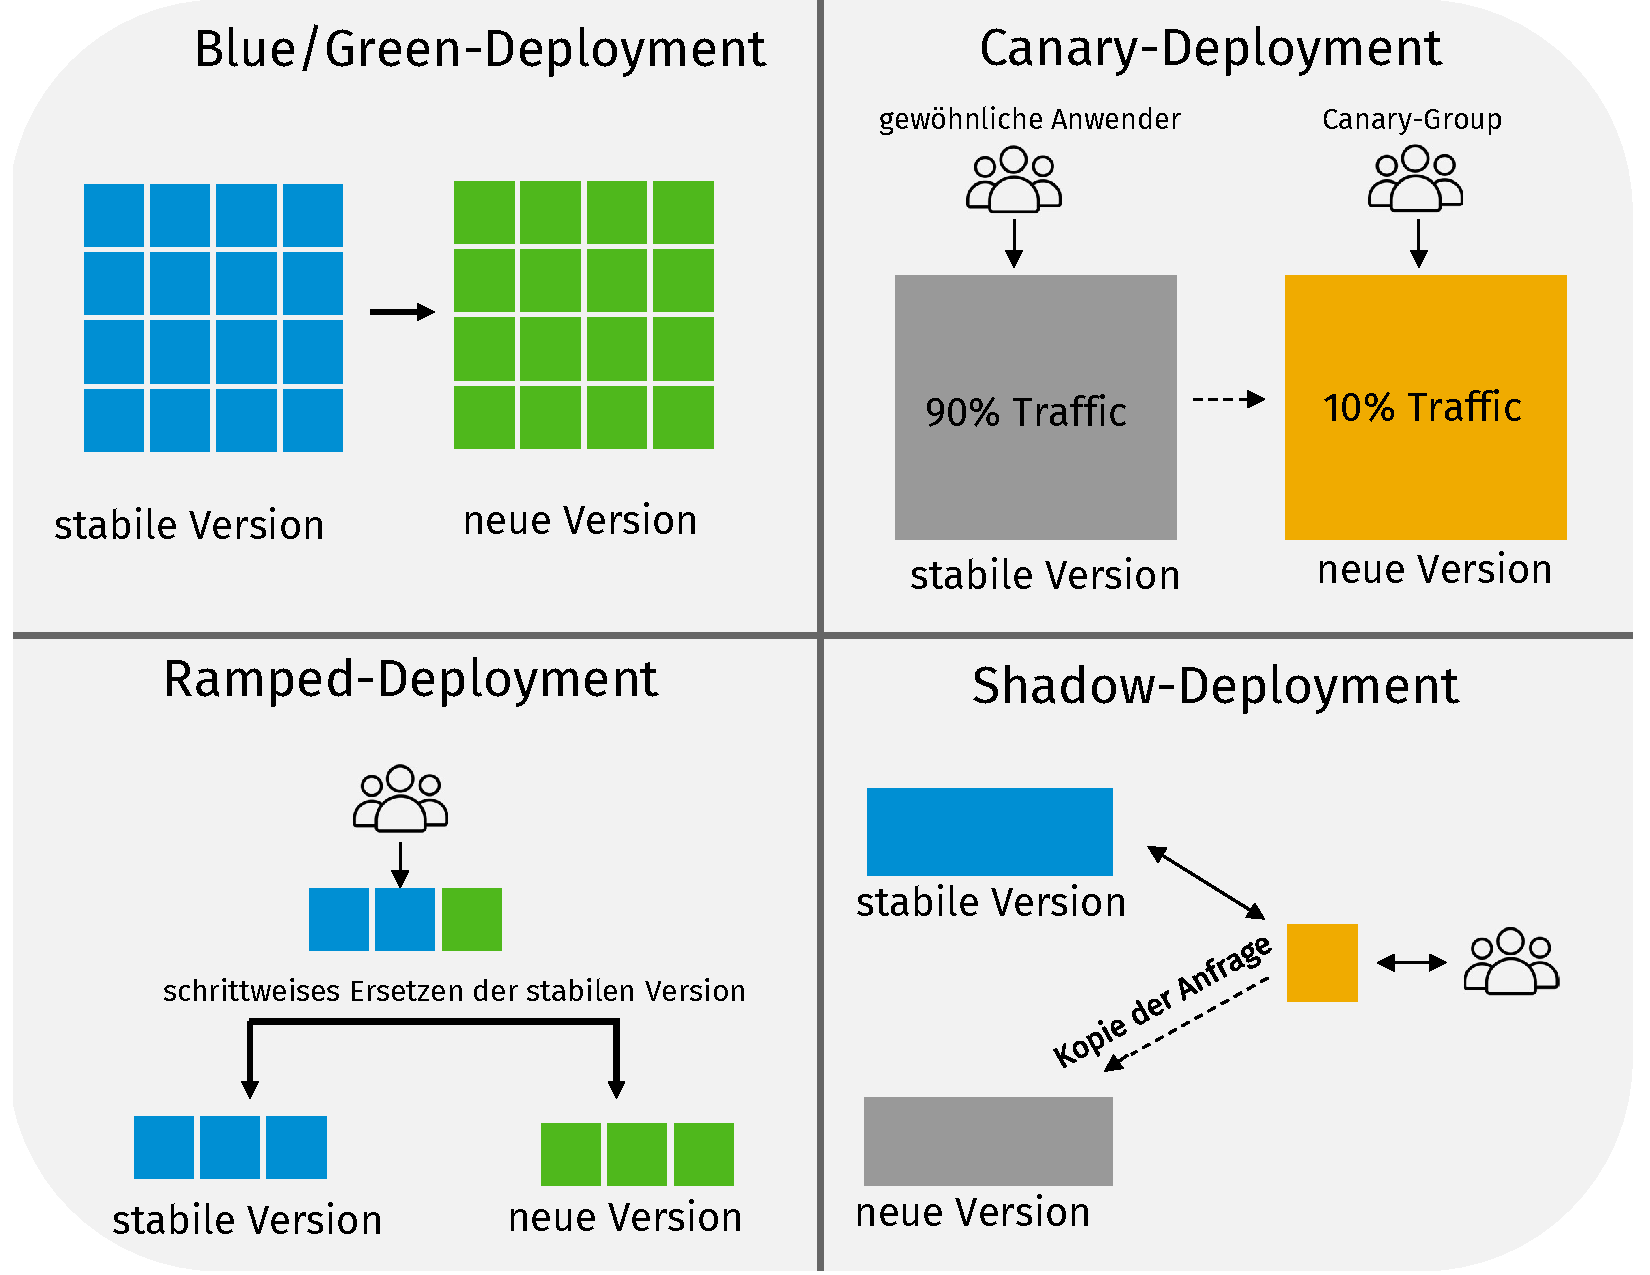
\includegraphics{Deployment_Strategies}}
		\caption[Strategien zur Bereitstellung von Software]{Strategien zur Bereitstellung von Software.\\ In Anlehnung an Ugochi \cite{Ugochi.20220503}.}
		\label{fig:DS}
	\end{figure}
\end{center}
\vspace*{-10mm}
Eine häufig verwendete Deployment-Strategie ist dabei das \textit{Blue/Green-Deployment}. Hierbei wird neben der stabilen aktuellen Anwendung (\textit{Blaue Version}) ebenfalls eine Instanz der neuen Anwendung (\textit{Grüne Version}) betrieben. Nutzeranfragen werden dabei von dem Lastenverteilungsservice (\textit{Load-Balancer}) erst nach Validierung aller Tests umgeschalten. Dazu gehören neben den in der CI/CD-Pipeline definierten Tests ebenfalls Überprüfungen der Qualitätssicherung. Diese umfassen manuelle Tests, in welchen Funktionen, Benutzeroberfläche sowie die Anwenderfreundlichkeit überprüft werden \cite{Ugochi.20220503}. Im Gegensatz zum Blue/Green-Deployment, bei welchem eine neue Version simultan für die gesamte Nutzerbasis zur Verfügung gestellt wird, gewährleistet das \textit{Canary-Deployment} eine restriktivere Nutzlastumleitung. Hierfür wird die neue Anwendungsversion vorerst einer überschaubaren Nutzeranzahl (\textit{Canary-Gruppe}) bereitgestellt. Dabei sollte die zusammengestellte Canary-Gruppe die Gesamtnutzerbasis möglichst gut repräsentieren. Anhand des Canary-Traffics soll der fehlerfreie Betrieb neuer Anwendungen überprüft und ggf. Anpassungen vorgenommen werden, bevor diese der gesamten Nutzerbasis zur Verfügung gestellt werden \cite{Ugochi.20220503}. Für Anwendungen auf einer kritischen IT-Infrastruktur wird i.d.R. die \textit{Ramped-Deployment-Strategie} verwendet. Diese ermöglicht eine präzise Kontrolle horizontal skalierter Services. Bei einer horizontalen Skalierungen erfolgt die Replizierung eine identischen Service-Instanzen, wodurch die Ausfallsicherheit einer Anwendung optimiert werden kann. Die neue Softwareversion wird während des Ramped-Deployment-Prozesses schrittweise auf die horizontalen Instanzen ausgerollt. Dabei werden die ersten aktualisierten Instanzen lediglich für bestimmte Anwender, eine sog. \textit{Ramped-Gruppe}, bereitgestellt. Dabei soll das von dieser Anwendergruppe zur Verfügung gestellte Feedback während zukünftiger Planungsprozesse berücksichtigt werden \cite{Ugochi.20220503}. Eine aufwendigere, jedoch risikoärmere Bereitstellungsstrategie stellt das \textit{Shadow-Deployment} dar. Dabei wird neben der Instanz der aktuellen Version ebenfalls ein sog. \textit{Shadow-Model} auf der Infrastruktur betrieben. Das Shadow-Model verwaltet die neue Version der Anwendung, kann jedoch nicht unmittelbar von den Nutzern aufgerufen werden. Diese Instanz stellt ein hinter der stabilen Version gelagertes Schattenmodell dar. Benutzeranfragen werden von dem Load-Balancer stets auf die aktuelle Version der Instanz weitergeleitet, verarbeitet und beantwortet. Gleichzeitig wird eine Kopie dieser Anfrage an das Shadow-Model weitergeleitet und von diesem prozessiert. Die Shadow-Modell-Verarbeitung des in der Produktionsumgebung abgewickelten Netzwerkverkehrs ermöglicht den Entwicklern somit eine anwendungsbezogene Überprüfung entwickelter Features \cite{Ugochi.20220503}. 